\section{How common are split votes?}
\label{leaderelection:split:rate}

The previous section analyzed the performance of normal elections when
no split vote occurs. In practice, two or more candidates may time out
at similar times, leading to split votes.  Split votes cause additional
election timeout delays, and if they occur too frequently, they can
impact election performance dramatically. This section first analyzes
split votes under a simplifying assumption that network latencies are
constant, then subsequently relaxes this assumption.

\subsubsection{Split vote rate with fixed latency}

\begin{figure}
\centering
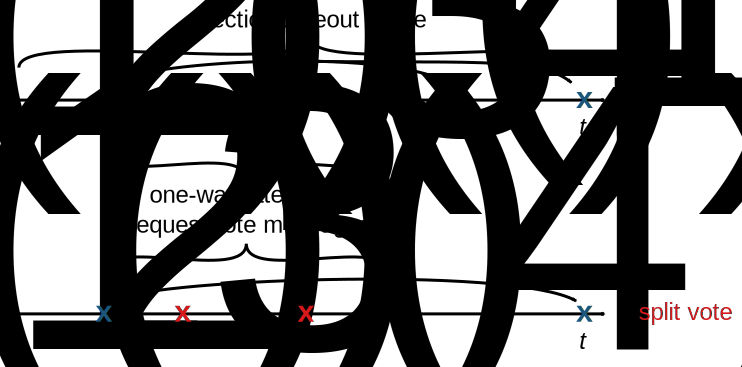
\includegraphics[scale=.5]{leaderelection/splitvotediagram}
\vcaption[split vote example with fixed latency]{
These examples show two similar elections in a five-server cluster when
one server has failed and network messages have a fixed latency. Each
server's random timeout value is shown on the timelines, where $t_{(1)}$
is the smallest value chosen, $t_{(2)}$ is the second-smallest, and so
on. In the top election, the first server is able to collect votes from
itself, the third server, and the fourth server. However, in the bottom
election, its RequestVote RPC cannot reach the third server in time
before that server times out; thus, the election ends in a split vote.
}
\label{fig:leaderelection:theory:splitvotediagram}
\end{figure}

Split votes can be calculated more simply if network latencies are
fixed. Let the constant $l$ be the one-way latency between any two
servers in the cluster, measured as a fraction of the election timeout
range.
Because of the fixed network latency,
the first server to time out is guaranteed to get the
votes of all servers that don't time out within $l$ of it, and it will
receive none of the votes of the other servers, who will each vote for
themselves.
The probability of a split vote is thus the probability that
too many candidates time out within $l$ of each other. For example,
consider a five-server cluster in which only four servers are available.
As illustrated in Figure~\ref{fig:leaderelection:theory:splitvotediagram},
if only two servers time out within $l$ of each other, the earliest server
will be able to collect votes from itself and the other two servers and
become leader. However, if three servers time out within $l$, then the
earliest server will only be able to reach one other server in time to
receive its vote, so the vote is split.

To derive a general formula for when split votes
occur, let $c$ denote the number of servers that time out within $l$ of
each other and let $n$ be the size of the full cluster.
The first server will get its own vote plus votes from the $s-c$ servers
that time out at least $l$ time after the first. Thus, a split vote
occurs when the following condition holds:
\begin{align*}
\text{votes needed}              &> \text{votes available to earliest server} \\
\Big\lfloor \dfrac{n}{2} \Big\rfloor + 1 &> 1 + (s - c) \\
c &> s - \Big\lfloor \frac{n}{2} \Big\rfloor
\end{align*}

How often split votes occur thus depends on how often at least $c$ servers
timeout within $l$ of each other. Let $D_{c,s} = T_{(c)} - T_{(1)}$,
where $T_{(i)}$ is a random variable representing the timeout of the
$i$-th of $s$ servers in sorted order; $D_{c,s}$ is the time after the
first server times out that the $c^\text{th}$ server times out. The
probability of split votes is then $\Pr(D_{c,s} < l)$, where $c$ is
determined by the formula given above ($s - \Big\lfloor \dfrac{n}{2}
\Big\rfloor + 1$).

We now derive the CDF for $D_{c,s}$, denoted $\Pr(D_{c,s} \leq l)$.
Suppose the first server times out at $t$.
%
First, if $t < 1-l$,
each of the following servers times out within $l$ time after $t$ with probability
$\dfrac{l}{1-t}$.
The probability that the second through $c^\text{th}$ servers time out
within $l$ time after $t$, and the remaining $s-c$ servers do not, is given by:
\begin{align*}
& \dbinom{s-1}{c-1}
  \left(\frac{l}{1-t}\right)^{c-1}
  \left(\frac{1-t-l}{1-t}\right)^{s-c}
\end{align*}
\noindent
%
Instead, if $t \geq 1-l$, then any server that times out after the first
must time out within $l$ time of $t$. Thus, all $s$ servers will
time out within $l$ of the first with probability $1$, and the
probability that any server does not timeout within $l$ of the first is
$0$. Putting this together, we can now derive the CDF:
%
\begin{align*}
\Pr(D_{c,s} \leq l)
%
 &= \mathlarger{\sum_{k=c}^s} \left(
\begin{aligned}
     &\int_0^{1-l}
     \Pr(\text{exactly $k$ servers time out in $t$ to $(t+l)$ range} \, | \, M_s=t)
     f_{M_s}(t) \, dt \, +
     \\
     &\int_{1-l}^1
     \Pr(\text{exactly $k$ servers time out in $t$ to $(t+l)$ range} \, | \, M_s=t)
     f_{M_s}(t) \, dt
\end{aligned}
\right) \displaybreak[0]\\
%
 &= \mathlarger{\sum_{k=c}^s}
     \left(
     \int_0^{1-l}
     \Pr(\text{exactly $k$ servers time out in $t$ to $(t+l)$ range} \, | \, M_s=t)
     f_{M_s}(t) \, dt
    \right) \, + \\
 &\quad \int_{1-l}^1 f_{M_s}(t) \, dt
  \displaybreak[0]\\
%
 &= \mathlarger{\sum_{k=c}^s}
     \left(
     \int_0^{1-l}
     \dbinom{s-1}{k-1}
     \left(\frac{l}{1-t}\right)^{k-1}
     \left(\frac{1-t-l}{1-t}\right)^{s-k}
     f_{M_s}(t) \, dt
    \right) \, + \\
 &\quad \int_{1-l}^1 f_{M_s}(t) \, dt
  \displaybreak[0]\\
%
 &= \mathlarger{\sum_{k=c}^s}
     \dbinom{s-1}{k-1}
     \left(
     \int_0^{1-l}
     \left(\frac{l}{1-t}\right)^{k-1}
     \left(\frac{1-t-l}{1-t}\right)^{s-k}
     s
     (1-t)^{s-1} \, dt
    \right) \, + \\
 &\quad \int_{1-l}^1 s (1-t)^{s-1} \, dt
  \displaybreak[0]\\
%
 &= \mathlarger{\sum_{k=c}^s}
     \dbinom{s-1}{k-1}
     \left. \left(
     -\frac{s}{s-k+1}
     l^{k-1}
     \left(1-t-l\right)^{s-k+1}
    \right) \right|_{t=0}^{1-l}
     \, + \\
 &\quad \mathlarger{\left. \left( -(1-t)^s \right)
\right|_{t=1-l}^1}
  \displaybreak[0]\\
%
 &= \left( \mathlarger{\sum_{k=c}^s}
     \dbinom{s-1}{k-1}
     \frac{s}{s-k+1}
     l^{k-1}
     (1-l)^{s-k+1}
    \right)
     \, + l^s
 \displaybreak[0] \\
%
 &= \left( \mathlarger{\sum_{k=c}^s}
     \frac{(s-1)! (s)}{(k-1)!(s-k)! (s-k+1)}
     l^{k-1}
     (1-l)^{s-k+1}
     \right)
     \, + l^s
    \displaybreak[0] \\
%
 &= \left(\mathlarger{\sum_{k=c}^s}
     \frac{s!}{(k-1)!(s-k+1)!}
     l^{k-1}
     (1-l)^{s-k+1}
     \right)
     \, + l^s
    \displaybreak[0] \\
%
 &= \left(\mathlarger{\sum_{k=c}^s}
     \dbinom{s}{k-1}
     l^{k-1}
     (1-l)^{s-k+1}
     \right)
     \, + l^s
    \displaybreak[0] \\
%
 &= \left(\mathlarger{\sum_{k=c-1}^{s-1}}
     \dbinom{s}{k}
     l^k
     (1-l)^{s-k}
     \right)
     \, + l^s
    \displaybreak[0] \\
%
 &= \mathlarger{\sum_{k=c-1}^s}
     \dbinom{s}{k}
     l^k
     (1-l)^{s-k}
    \displaybreak[0]
\end{align*}
%
(The CDF somewhat resembles a binomial distribution, which hints that
there may exist an easier derivation.)

For example, consider a five-server
cluster with four available servers ($s=4$). A split vote will occur if the
earliest three servers time out within $l$ of each other ($c=3$). If the
election timeout range is \SI{100}{\milli\second},
the earliest three servers will time
out within $l$ of each other, resulting in a split vote:
\begin{compactitem}
\item In about 0.06\% of elections, if the one-way network latency is
\SI{1}{\milli\second},
$\Pr(D_{3,4} \leq .01)$;
\item In about 5.2\% of elections, if the one-way network latency is
\SI{10}{\milli\second}, $\Pr(D_{3,4} \leq .1)$; and
\item In about 18.1\% of elections, if the one-way network latency is
\SI{20}{\milli\second}, $\Pr(D_{3,4} \leq .2)$.
\end{compactitem}

\begin{figure}
\centering
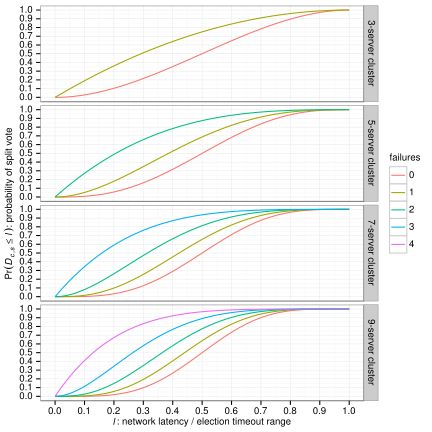
\includegraphics{leaderelection/distance}
\vspace{-2ex}
\vcaption[split vote probability with fixed network latency]{
The graphs show the likelihood of split votes for various cluster
sizes and numbers of server failures, given a fixed network latency $l$.
Each graph shows a different full cluster size, and the curves on each
graph show different numbers of failed servers in that cluster.
Each value represents the likelihood that a split vote will occur
because the first $c$ of the $s$ servers timed out within $l$ of each
other, where $c$ is determined by $s - \Big\lfloor \dfrac{n}{2}
\Big\rfloor + 1$.
For example, a five-server
cluster with two failures and $l=0.2$ will see about half of
elections end in split votes.
}
\label{fig:leaderelection:theory:distance}
\end{figure}


Figure~\ref{fig:leaderelection:theory:distance} graphs the CDF formula for
a range of cluster sizes. The first thing to observe is that failures
have a very large effect on split vote rates, especially if the cluster
is down to a bare majority of its original members. For example, a
five-server cluster
with $l=0.2$ will encounter less than 20\% split votes after one
failure;
if the same cluster encounters a second failure, about half of election
terms will encounter split votes. To prepare for worst-case scenarios,
the election timeout range should be set to produce tolerable values
when a bare majority of the cluster is available.

Second,
larger clusters experience fewer split votes with the same number of
failures, but they experience an even larger worst-case split vote rate
as a result of being able to tolerate more failures. For example, a
nine-server cluster with $l=0.2$ will experience only about a
15\% rate of
split votes after two failures (compare with 50\% for a five-server
cluster). However, when it is down to its bare majority with four
failures, the nine-server cluster will experience a nearly 70\% split vote rate.

Third, keeping the number of available servers constant, larger full
cluster sizes will have more split votes. For example, with $l=0.2$, a
nine-server cluster with six available servers will experience about a
35\% rate split votes; a seven-server cluster with six available servers will
experience only about a 10\% rate split votes. This is because larger full
clusters require more votes to win an election; fewer candidates need to
time out within $l$ of each other in order to produce a split vote.

Finally, the graphs suggest that choosing an election timeout range of
10--20 times the one-way network latency (so $l=0.1$) will result in low split
vote rates in all clusters, assuming network latencies are nearly
constant. With this setting, a nine-server cluster that has experienced
four failures will encounter 40\% split votes, and most typical clusters
will encounter much fewer. Smaller election timeouts (larger $l$ values)
may also work in many deployments, but they should be tested more
carefully to make sure.

\subsubsection{Split vote rate with variable latency}

When network latency is variable, calculating split vote rates is more
complicated. The problem is that a RequestVote message sent by one
server can overtake a RequestVote message sent earlier by a different
server. Thus, the first server to time out is no longer guaranteed to
collect all of the votes of servers that do not vote for themselves.
The first server is still the most likely candidate to win, by virtue of
sending requests for votes first, but its advantage depends on how much
earlier it timed out. Thus, with variable latency, we intuitively expect
somewhat higher rates of split votes (there is more competition).

\begin{figure}
\centering
\includegraphics{leaderelection/splits.pdf}
\vspace{-3ex}
\vcaption[split vote probability with variable network latency]{
The contour graphs show split vote rates for various cluster sizes and
numbers of failed servers. Each narrow contour line denotes a 1\%
increase in the probability of split votes; each medium contour line
denotes a 10\% increase; the thick contour line visible in some graphs
denotes the 50\% barrier. Split votes are always
0\% at the origin,
where messages are instantaneous. The points on the $x$ axis, where the
latency range is zero, correspond to the split vote rates with fixed
latencies in Figure~\ref{fig:leaderelection:theory:distance}.
\\
For example, the probability of a split vote for a five-server cluster
after one failure can be found in the graph in the second column and
second row. When latencies are chosen randomly and uniformly between 0.1
and 0.2, the point with a
minimum latency of 0.1 and a latency range of 0.1 reveals, by counting
contour lines, that the split vote rate is about 16\%. With two
failures, the probability of a split vote in the same cluster is nearly
40\%.
}
\label{fig:leaderelection:theory:splitvotes}
\end{figure}

Rather than model this mathematically, we used a small simulation. Each
run followed the following steps (before optimization):
%
\begin{enumerate}
%
\item Assign random timeouts to each of $s$ servers.
%
\item If a server has not voted by the time it times out, it votes for
itself and schedules RequestVote messages to be delivered to other
servers after random latencies.
%
\item If any server collects a majority of votes, the election term is
considered successful; otherwise, it is considered a split vote.
%
\end{enumerate}
%
After \num{10000} runs, the fraction of split votes was calculated.

Figure~\ref{fig:leaderelection:theory:splitvotes} shows the split vote
rates for messages with uniform random latencies in the range
$[l_\text{min},l_\text{max}]$, as calculated by the simulation.
(Uniform random latencies may not be a realistic distribution, but they
are the simplest case and can help with estimating more complex
distributions.)
The overall conclusion from these graphs is the same as
with fixed latency: more failures result in significantly higher split
vote rates.

In clusters with only a bare majority of servers available (the bottom
graph in each column), the contour lines are very linear with a slope of
about $-2$: they have about the same split vote rate when keeping the
average network latency constant. This indicates that the split vote
rates for bare-majority clusters
can be accurately approximated with our fixed latency model using
the average of the variable latency range. For example in a nine-server
cluster with four failures, a variable latency chosen randomly from the
range $[0.1, 0.2]$ results in a similar split vote rate as a fixed
latency of $0.15$.

In clusters with fewer failures, the contour lines aren't always linear,
and they typically have less slope in general (they are flatter). For
example, in a five-server cluster with no failures, a variable latency
between 0.1 and 0.2 has a similar split vote rate as a fixed latency of
about 0.2 (the slope of the contour lines is only about $-1$).
Typically, split vote rates can be bounded with our fixed latency model
using the maximum of the variable latency range. This is true for about
78\% of the data points shown in the figure; however, this approximation
works least well for large clusters with few failures, as these contour
lines are most curved.
